\chapter{はじめに}

\section{研究の背景}
ドローンとは,無人で遠隔操作や自動制御によって飛行できる航空機の総称のことである.ドローンの始まりは図1.1に示す軍事用に偵察や攻撃用に作られたプレデターが始まりである.近年,図1.2に示す宅配サービスや図1.3に示す農薬を撒く農業用,図1.4図1.5に示す空撮,水中撮影,図1.6に示す掌に収まるくらいの小型用,図1.7に示す娯楽等のドローンが普及してきた.3つ以上のメインローターを持つヘリコプターをマルチコプターと呼び,その中から4つのメインローターを持つクアッドコプター図1.8について研究する.室内で使うことのできるマルチコプターは多くない.

\begin{figure}[htbp]
  \begin{center}
    \includegraphics[width=100mm]{img/図1.jpg}
    \end{center}
  \caption{プレデタ―}
 \label{fig:robot}
\end{figure}

\begin{figure}[htbp]
  \begin{center}
    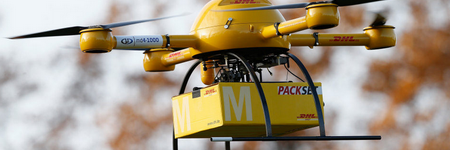
\includegraphics[width=100mm]{img/ドローンの商業利用.png}
    \end{center}
  \caption{商業用}
 \label{fig:robot}
\end{figure}

\begin{figure}[htbp]
  \begin{center}
    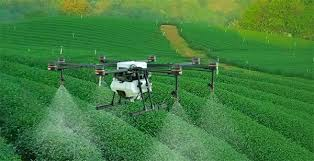
\includegraphics[width=100mm]{img/images.jpg}
    \end{center}
  \caption{農業用}
 \label{fig:robot}
\end{figure}

\begin{figure}[htbp]
  \begin{center}
    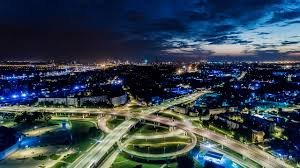
\includegraphics[width=100mm]{img/空撮.jpg}
    \end{center}
  \caption{空撮}
 \label{fig:robot}
\end{figure}

\begin{figure}[htbp]
  \begin{center}
    \includegraphics[width=100mm]{img/図2.jpg}
    \end{center}
  \caption{水中撮影用}
 \label{fig:robot}
\end{figure}

\begin{figure}[htbp]
  \begin{center}
    \includegraphics[width=100mm]{img/図3.jpg}
    \end{center}
  \caption{小型の娯楽用}
 \label{fig:robot}
\end{figure}

\begin{figure}[htbp]
  \begin{center}
    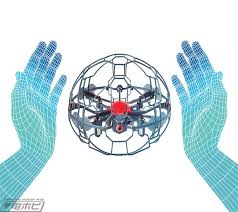
\includegraphics[width=100mm]{img/ダウンロード.jpg}
    \end{center}
  \caption{娯楽用}
 \label{fig:robot}
\end{figure}

\begin{figure}[htbp]
  \begin{center}
    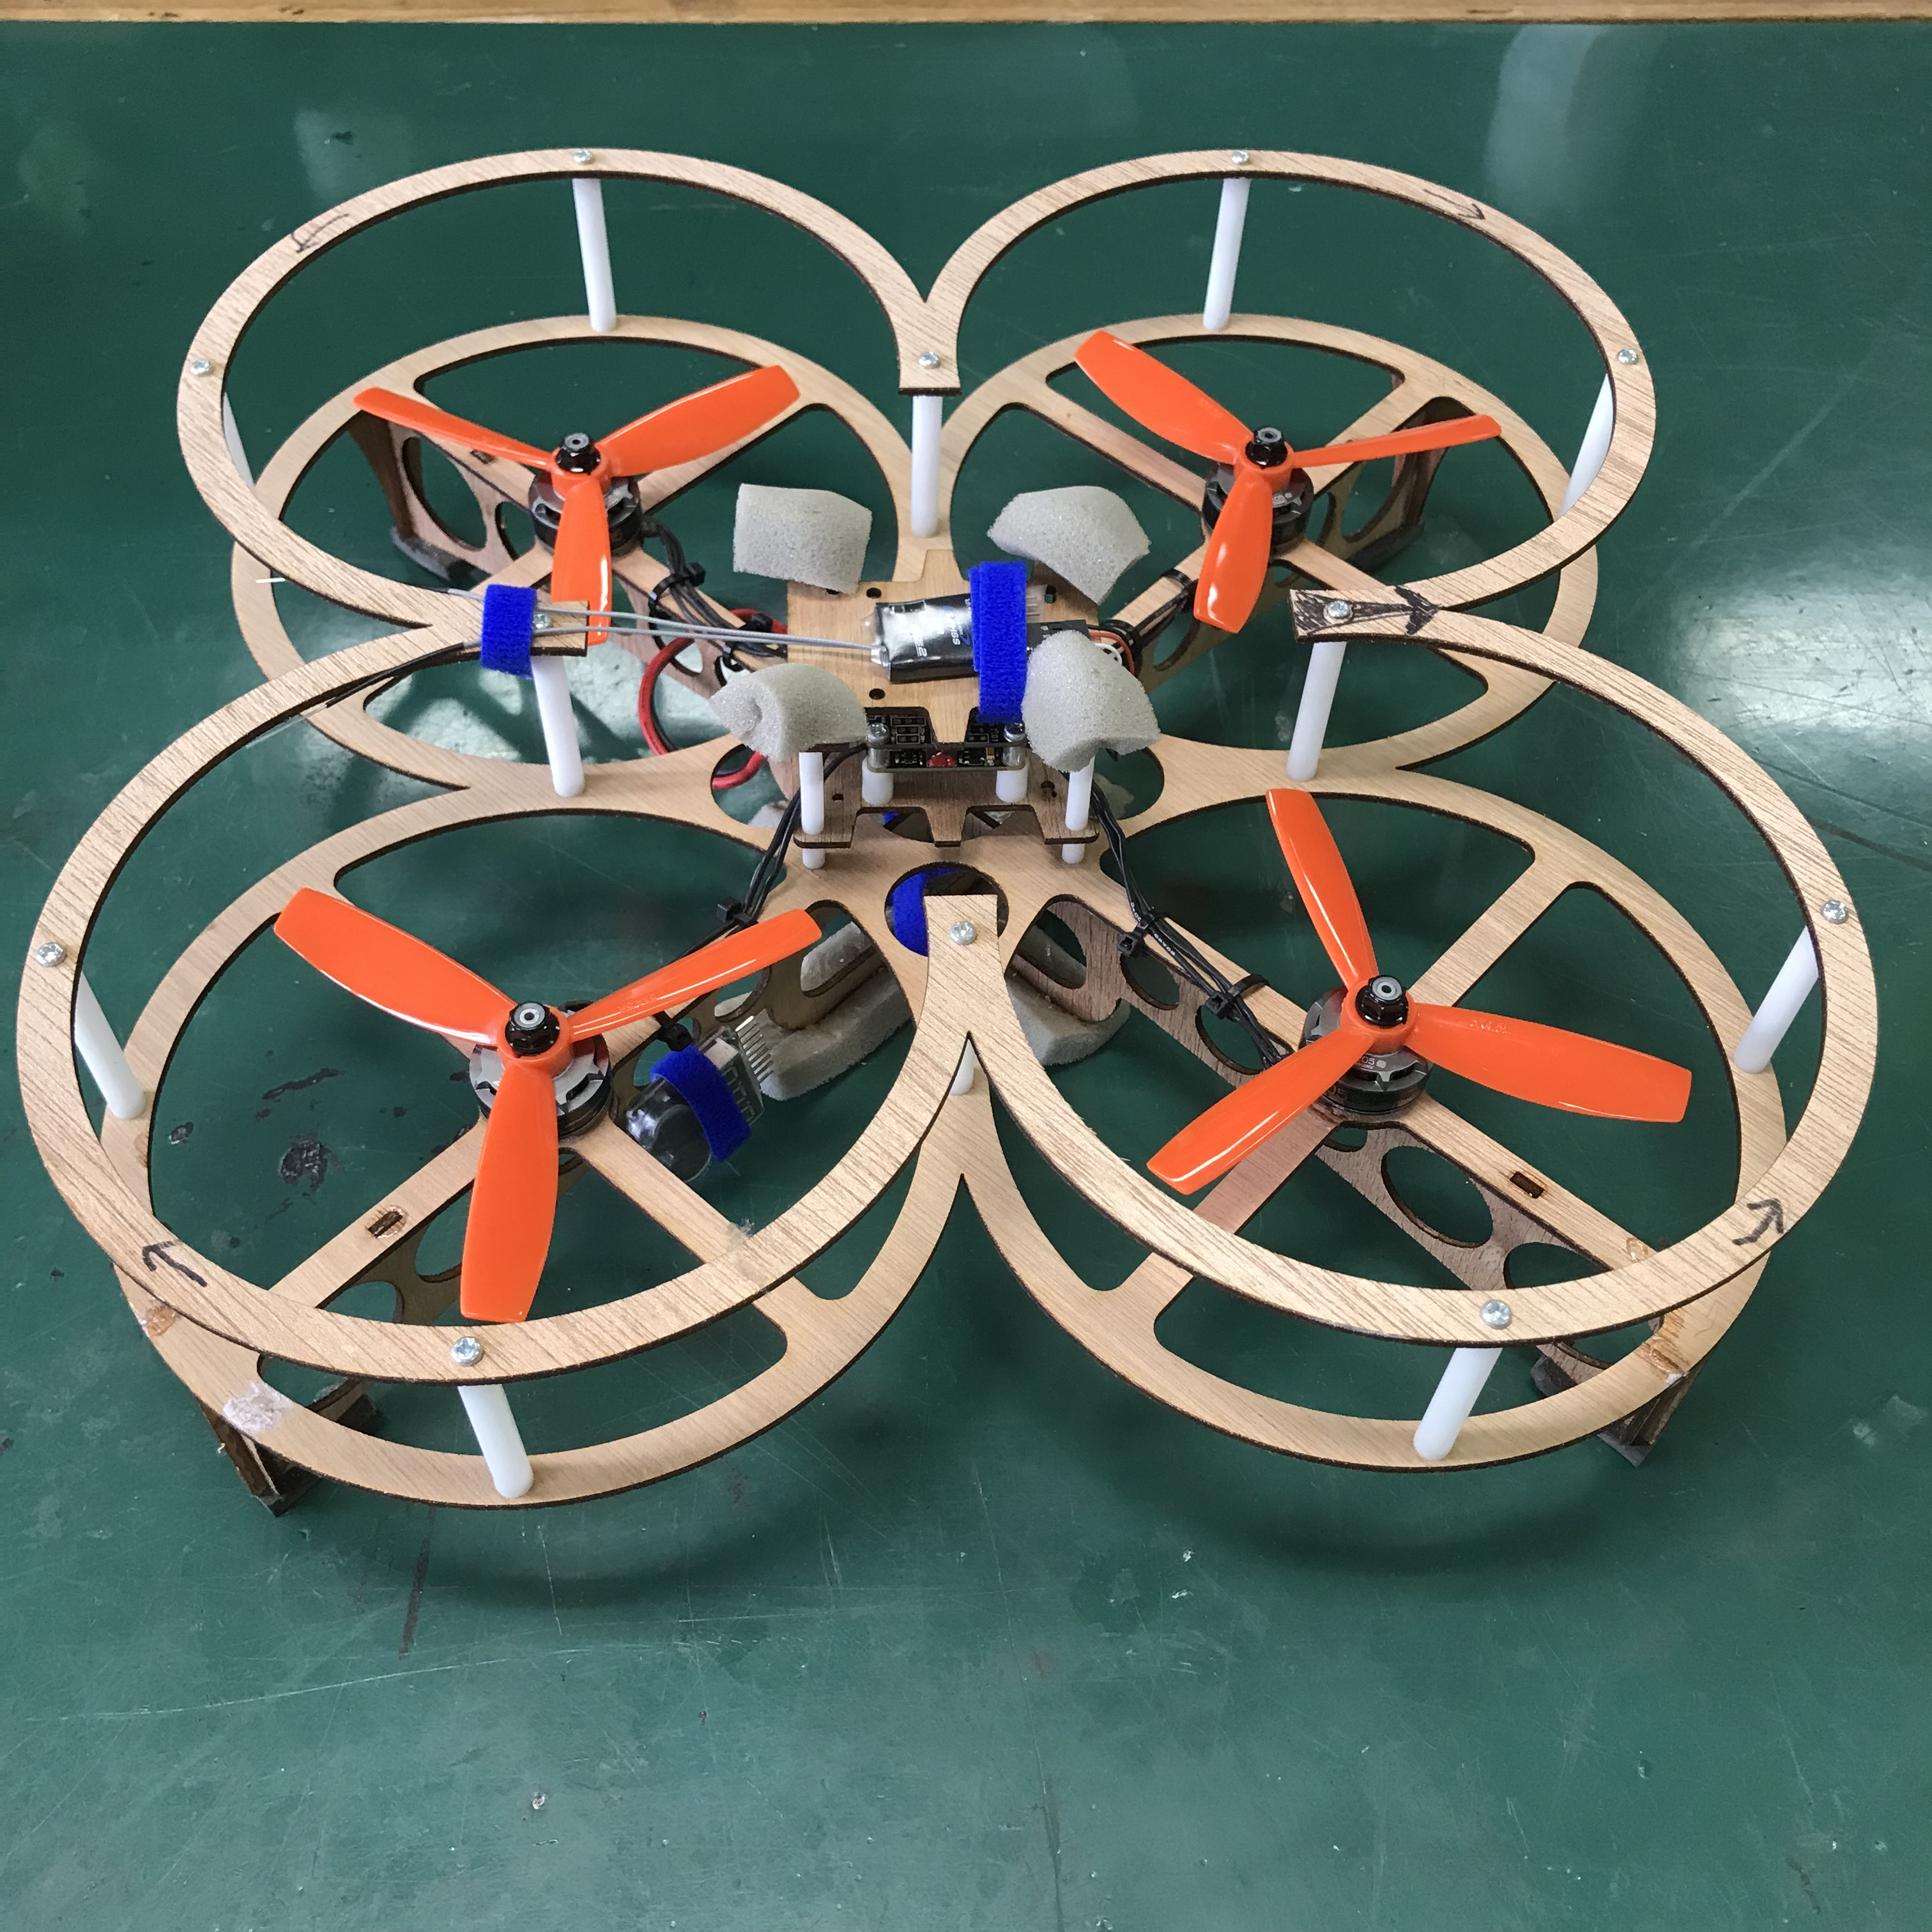
\includegraphics[width=100mm]{img/drone.jpeg}
    \end{center}
  \caption{クアッドコプター}
 \label{fig:robot}
\end{figure}

\section{研究の目的}

自動制御の課題がいくつかあり,その中に高度制御を利用した自動着陸があり,課題を達成するため高度制御について研究する.

\section{本論文の構成}
1章では,本研究の背景と簡略化した概要を示す.
2章では飛行ロボコンについて述べる.
3章ではマルチコプター運動方程式について述べる.
4章では高度制御について述べる.

5章では高度制御のシミュレーション実験について述べる.
6章で考察を述べる.
7章で最後に本実験のまとめを述べる.